Consider the lines 
%
\begin{enumerate}
%\begin{multicols}{2}
\item
\begin{align}
\begin{split}
\myvec{2 & 3 }\vec{x}&=8
\\
\myvec{3 & 2 }\vec{x}&=4 \label{linform/2/9/1.0.1} 
\end{split}
\end{align}
The above equations can be expressed as the matrix equation
\begin{align}
\myvec{2 & 3\\3 & 2} \vec{x} = \myvec{8\\4}
\end{align}
%
The augmented matrix for the above equation is row reduced as follows
\begin{align}
\myvec{2 & 3 & 8\\3 & 2 & 4} 
\xleftrightarrow {R_1\leftarrow \frac{R_1}{2}}\myvec{1 & \frac{3}{2} & 4 & \\3 & 2 & 4} 
\\
%\myvec{1 & \frac{3}{2} & 4 \\3 & 2 & 4}
\xleftrightarrow {R_2\leftarrow R_2-3R_1}\myvec{1 & \frac{3}{2} & 4 \\0 & \frac{-5}{2} & -8}
\\
%\myvec{1 & \frac{3}{2} & 4 \\0 & 1 & \frac{16}{5}} 
\xleftrightarrow {R_2\leftarrow \frac{2R_2}{-5}}\myvec{1 & \frac{3}{2} & 4 \\0 & 1 & \frac{16}{5}}
\\
%\myvec{1 & 0 & \frac{-4}{5} \\0 & 1 & \frac{16}{5}} 
\xleftrightarrow {R_1\leftarrow  R_1-\frac {3R_2}{2}}\myvec{1 & 0 & \frac{-4}{5} \\0 & 1 & \frac{16}{5}}
\end{align}
%
$\because$ row reduction of the $2\times 3$ matrix
%
\begin{align}
\myvec{2 & 3 & 8\\3 & 2 & 4} \label{linform/2/9/2.0.7}
\end{align}
%
results in a matrix with 2 nonzero rows, its rank is 2. 
%
Similarly, the rank of the matrix 
\begin{align}
\myvec{2 & 3 \\3 & 2 } \label{linform/2/9/2.0.8}
\end{align}
%
is 2.
%
\begin{align}
\because Rank \myvec{2 & 3\\3 & 2} &= Rank\myvec{2 & 3 & 8\\3 & 2 & 4} \nonumber\\
 &=dim \myvec{2 & 3\\3 & 2}\nonumber\\
 &=2
\end{align}
$\therefore$ the lines in  \eqref{linform/2/9/1.0.1} intersect as can be seen from Fig.     \ref{linform/2/9/fig:INTERSECTING LINES.}.
\begin{figure}[!ht]
    \centering
    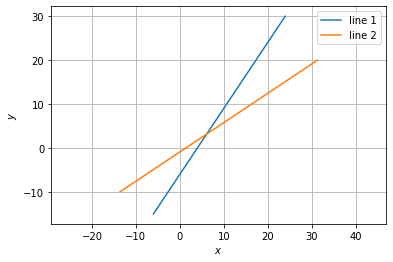
\includegraphics[width=\columnwidth]{solutions/su2021/2/9/FIGURES/INTERSECTING_LINES.png}
    \caption{INTERSECTING LINES.}
    \label{linform/2/9/fig:INTERSECTING LINES.}
\end{figure} 

\item
\begin{align}
\begin{split}
\myvec{2 & 3 }\vec{x}&=8
\\
\myvec{4 & 6 }\vec{x}&=16 \label{linform/2/9/1.0.2}
\end{split}
\end{align}

The above equations can be expressed as the matrix equation
\begin{align}
\myvec{2 & 3\\4 & 6} \vec{x} = \myvec{8\\16}
\end{align}
%
The augmented matrix for the above equation is row reduced as follows
\begin{align}
\myvec{2 & 3 & 8\\4 & 6 & 16 } 
\xleftrightarrow {R_1\leftarrow \frac{R_1}{2}}\myvec{1 & \frac{3}{2} & 4\\4 & 6 & 16 }
\\
%\myvec{1 & \frac{3}{2} & 4 \\0 & 0 & 0 
\xleftrightarrow {R_2\leftarrow R_2-4R_1}\myvec{1 & \frac{3}{2} & 4 \\0 & 0 & 0}
\\
\end{align}
%
$\because$ row reduction of the $2\times 3$ matrix
%
\begin{align}
\myvec{2 & 3 & 8\\4 & 6 & 16}
\end{align}
%
results in a matrix with 1 nonzero rows, its rank is 1. 
%
Similarly, the rank of the matrix 
\begin{align}
\myvec{2 & 3 \\4 & 6 } 
\end{align}
%
is also 1.
%
\begin{align}
\because Rank \myvec{2 & 3\\4 & 6} &= Rank\myvec{2 & 3 & 8\\4 & 6 & 16}=1\nonumber\\
&= dim\myvec{2 & 3\\4 & 6}=1
\end{align}
$\therefore$ the  lines in \eqref{linform/2/9/1.0.2} coincide as can be seen from Fig.     \ref{linform/2/9/fig:COINCIDENT LINES.}.

\begin{figure}[!ht]
    \centering
    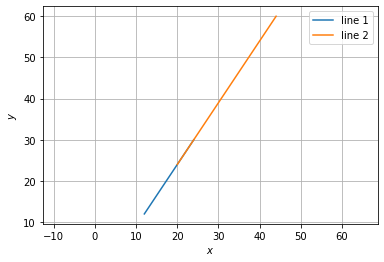
\includegraphics[width=\columnwidth]{solutions/su2021/2/9/FIGURES/COINCIDENT_LINES.png}
    \caption{COINCIDENT LINES}
    \label{linform/2/9/fig:COINCIDENT LINES.}
\end{figure} 

\item
\begin{align}
\begin{split}
\myvec{2 & 3 }\vec{x}&=8
\\
\myvec{2 & 3 }\vec{x}&=4 \label{linform/2/9/1.0.3}
\end{split}
\end{align}
%\end{multicols}
The above equations can be expressed as the matrix equation
\begin{align}
\myvec{2 & 3\\2 & 3} \vec{x} = \myvec{8\\4}
\end{align}
%
The augmented matrix for the above equation is row reduced as follows
\begin{align}
\myvec{2 & 3 & 8\\2 & 3 & 4 } 
\xleftrightarrow {R_1\leftarrow \frac{R_1}{2}}\myvec{1 & \frac{3}{2} & 4\\2 & 3 & 4 }
\\
%\myvec{1 & \frac{3}{2} & 4 \\0 & 0 & -4
\xleftrightarrow {R_2\leftarrow R_2-2R_1}\myvec{1 & \frac{3}{2} & 4 \\0 & 0 & -4}
\\
\end{align}
%
$\because$ row reduction of the $2\times 3$ matrix
%
\begin{align}
\myvec{2 & 3 & 8\\2 & 3 & 4}
\end{align}
%
results in a matrix with 2 nonzero rows, its rank is 2. 
%
Similarly, the rank of the matrix 
\begin{align}
\myvec{2 & 3 \\2 & 3 } 
\end{align}
%
is 1.
%
\begin{align}
\because Rank \myvec{2 & 3 \\2 & 3 } \ne Rank \myvec{2 & 3 & 8\\2 & 3 & 4}
\end{align}
$\therefore$ the  lines in \eqref{linform/2/9/1.0.3} are parallel as can be seen from Fig.  \ref{linform/2/9/fig: PARALLEL LINES.}.
%
\begin{figure}[!ht]
    \centering
   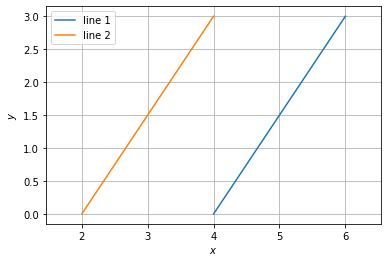
\includegraphics[width=\columnwidth]{solutions/su2021/2/9/FIGURES/PARALLEL_LINES.png}
    \caption{PARALLEL LINES}
    \label{linform/2/9/fig: PARALLEL LINES.}
\end{figure}    
\end{enumerate}

